\documentclass[10pt,journal,compsoc]{IEEEtran}

\usepackage[all,pdf]{xy}
\usepackage{tikz}
\usepackage{cite}
\usepackage{amsmath}
\usepackage{todonotes}
\usepackage{nicefrac}
\usepackage{lmodern,amssymb}
\usepackage{float}
\usepackage{graphicx}
\usepackage{caption}
\usepackage{subcaption}
\usetikzlibrary{positioning}

% Commands
\newcommand\smallO{
  \mathchoice
    {{\scriptstyle\mathcal{O}}}% \displaystyle
    {{\scriptstyle\mathcal{O}}}% \textstyle
    {{\scriptscriptstyle\mathcal{O}}}% \scriptstyle
    {\scalebox{.50}{$\scriptscriptstyle\mathcal{O}$}}%\scriptscriptstyle
  }

\interdisplaylinepenalty=2500

\newtheorem{theorem}{Theorem}
\newtheorem{lemma}{Lemma}
\newtheorem{definition}{Definition}

\hyphenation{op-tical net-works semi-conduc-tor}

\makeatletter
\def\endthebibliography{%
  \def\@noitemerr{\@latex@warning{Empty `thebibliography' environment}}%
  \endlist
}
\makeatother

\begin{document}

\title{Finding Lower Bounds for the Number of Comparison in Selection Algorithms}

\author{Josua Dörrer, Konrad Gendle, Johanna Hofmann, Julius von Smercek, Andreas Steding% <-this %
  \IEEEcompsocitemizethanks{\IEEEcompsocthanksitem Institut für Formale Methoden der
    Informatik (FMI)\protect\\
    Universität Stuttgart
  }}

\markboth{Bachelor-Forschungsprojekt}%
{Submission}

\IEEEtitleabstractindextext{%
  \begin{abstract}
    This research project aims to find worst case optimal comparison algorithms for selecting the
    i-th smallest of n elements of a set for n up to 15 with computer search.
  \end{abstract}

  \begin{IEEEkeywords}
    Selection, Pessimistic lower Bound, Partial Order Sets, Computer Search
  \end{IEEEkeywords}}


\maketitle

\IEEEdisplaynontitleabstractindextext


\IEEEpeerreviewmaketitle

\IEEEraisesectionheading{
  \section{Motivation}
  \label{sec:motivation}
} \IEEEPARstart{T}{he} problem of selecting the $i$-th smallest element in a list of $n$ elements is
a well known problem in computer science and called \textit{selection}. A first approach to solve
this can be achieved by sorting the list at first and selecting the $i$-th element. However, this
approach has a time complexity of $\mathcal{O}(n \cdot \log n)$. Putting more thought into this
problem one can find algorithms like the median of medians (Schöning \cite{Schoening1993}) or PICK
(Blum \cite{Blum1972}) and reduce the time complexity to $\mathcal{O}(n)$. Optimal algorithms are
known for any $n$ when $i$ is either one or two, but there is a significant performance gap finding
the median $i = \nicefrac{n}{2}$ from the best known algorithm with a time complexity of $2.97 \cdot
  n + \smallO(n)$ to the tightest known minimum of $2 \cdot n - \smallO(n)$.

Searching for optimal solutions is considerably difficult and the tightest known lower bounds
obtained by mathematical means soon exceed what is attainable by even rather intelligent search. An
approach to finding optimal algorithms is made by Gasarch, Kelly and Pugh \cite{Gasarch1996} who
introduced computer search to find optimal selection algorithms. On his website Kenneth Oksanen
\cite{Oksanen} published a computer search algorithm improving the previously known lower bounds
found by Gasarch et. al. However, the results are not published in a scientific journal and lack
explanation. This work will continue the work of Oksanen \cite{Oksanen} by confirming, improving and
expanding the values he found. It will reimplement some ideas of the algorithms Oksanen published
along with his found lower bounds and improve the computer search algorithms by researching the
benefits of different search strategies, adding $\alpha$-$\beta$-pruning and the exploitation of
compatible Posets. A quote from Miguel de Cervantes from Don Quijote will hold true for this
article: The journey is better than the inn. So buckle up.

\section{Fundamentals}
\subsection{Algorithms for Finding the $i$-th largest of $n$ elements}
\subsubsection{Sorting}
A baseline algorithm to select the $i$-th element in a list of $n$ values is to use a sorting
algorithm like merge sort or heap sort on the input data and then return the $i$-th element of the
now sorted list. The time complexity of this approach is essentially the runtime to sort the list.
For the sorting algorithms mentioned the time complexity is of $\mathcal{O}(n \cdot \log n)$

\subsubsection{Pivoting}
A better approach solving the selection problem can be achieved by using pivoting. The common idea
of the algorithms using pivoting is to promote an element from the input to a so called
\textit{pivot} element and use comparisons against this element to divide the remaining $n-1$ input
elements into two subsets. Let $L$ be the subset with elements less then the pivot element and $G$
the subset with elements greater than the pivot element. The algorithm can then determine whether to
search for the $i$-th element in the subset $L$ or the subset $G$. Using pivot algorithms like
Floyd-Rivest algorithm, a variation of quickselect, the runtime can be reduced to
$\mathcal{O}(\sqrt{n \cdot \log n})$. The first linear-time deterministic selection algorithm known
is  also commonly taught in computer science class is the median of medians. It partitions the input
data into sets of five in linear time. Then it calls itself on each of the sets to find the median
of these sets of five. The result is a algorithm that returns the median in $\mathcal{O}(n)$. In
practice the algorithm performs poorly compared to quickselect and is also slower than sorting the
list of moderate size due to its high constant factor. Better algorithms like quickselect or PICK
have a lower constant factor but all these algorithms share the same time complexity
$\mathcal{O}(n)$.
\todo{hier fehlt ein cite}
% https://en.wikipedia.org/wiki/Selection_algorithm#cite_note-knuth-14

\subsubsection{Lower and upper bounds}
The time complexity of $\mathcal{O}(n)$ of the mentioned algorithms is necessary, because the input
to these algorithm is a list of values in arbitrary order. Therefore the algorithm must look at all
the input values to determine a correct solution. If any of these input values will not be
considered it could be the one that should have been returned by the algorithm leading to wrong
results. Apart from this simple and straight forward argument, there is a considerable amount of
research on the exact number of comparisons required for selection, both in the randomized and
deterministic cases.

It has been found that selecting the $i$-th element of $n$ requires at least
$n+\min(i,n-i)-\mathcal{O}(1)$ comparisons, thus matching the average case of the Floyd-Rivest
algorithm up to his $\smallO(n)$ term. For deterministic algorithms it has also been shown that
\begin{eqnarray*}
  &\left (1 + H(i/n) \right ) \cdot n + \Omega(\sqrt n) \\
  &\text{with~} H(x) = x \cdot \log_2 \frac{1}{x} + (1-x) \log_2 \frac{1}{1-x}
\end{eqnarray*}
are required. An upper bound is been proposed by Blum, in the paper \textit{Time Bounds for
  Selection} it stated that no more than $5.430\dot{5} \cdot n$ comparisons are ever required.
Therefore selection is for sure in a time complexity of $\mathcal{O}(n)$ for best and worst-case.

\subsection{Partial Order}
To dive deeper into these algorithms the concept of partial orders needs to be introduced. A partial
order, often simply called a reflexive, weak, or non-strict partial order, is a homogeneous relation
$\leq$ on a set $P$ that satisfies reflexivity, anti symmetry, and transitivity. For any $a, b, c
  \in P$, it must adhere to the following conditions:

\begin{itemize}
  \item Reflexivity: $a \leq a$, meaning every element is related to itself.
  \item Antisymmetry: If $a \leq b$ and $b \leq a$, then $a = b$, implying no two distinct elements
        precede each other.
  \item Transitivity: If $a \leq b$ and $b \leq c$, then $a \leq c$.
\end{itemize}


A non-strict partial order is also known as an antisymmetric pre order.
%[\todo{cite:https://en.wikipedia.org/wiki/Partially_ordered_set}]

\subsection{Example}
\begin{figure}[h!]
  \centering
  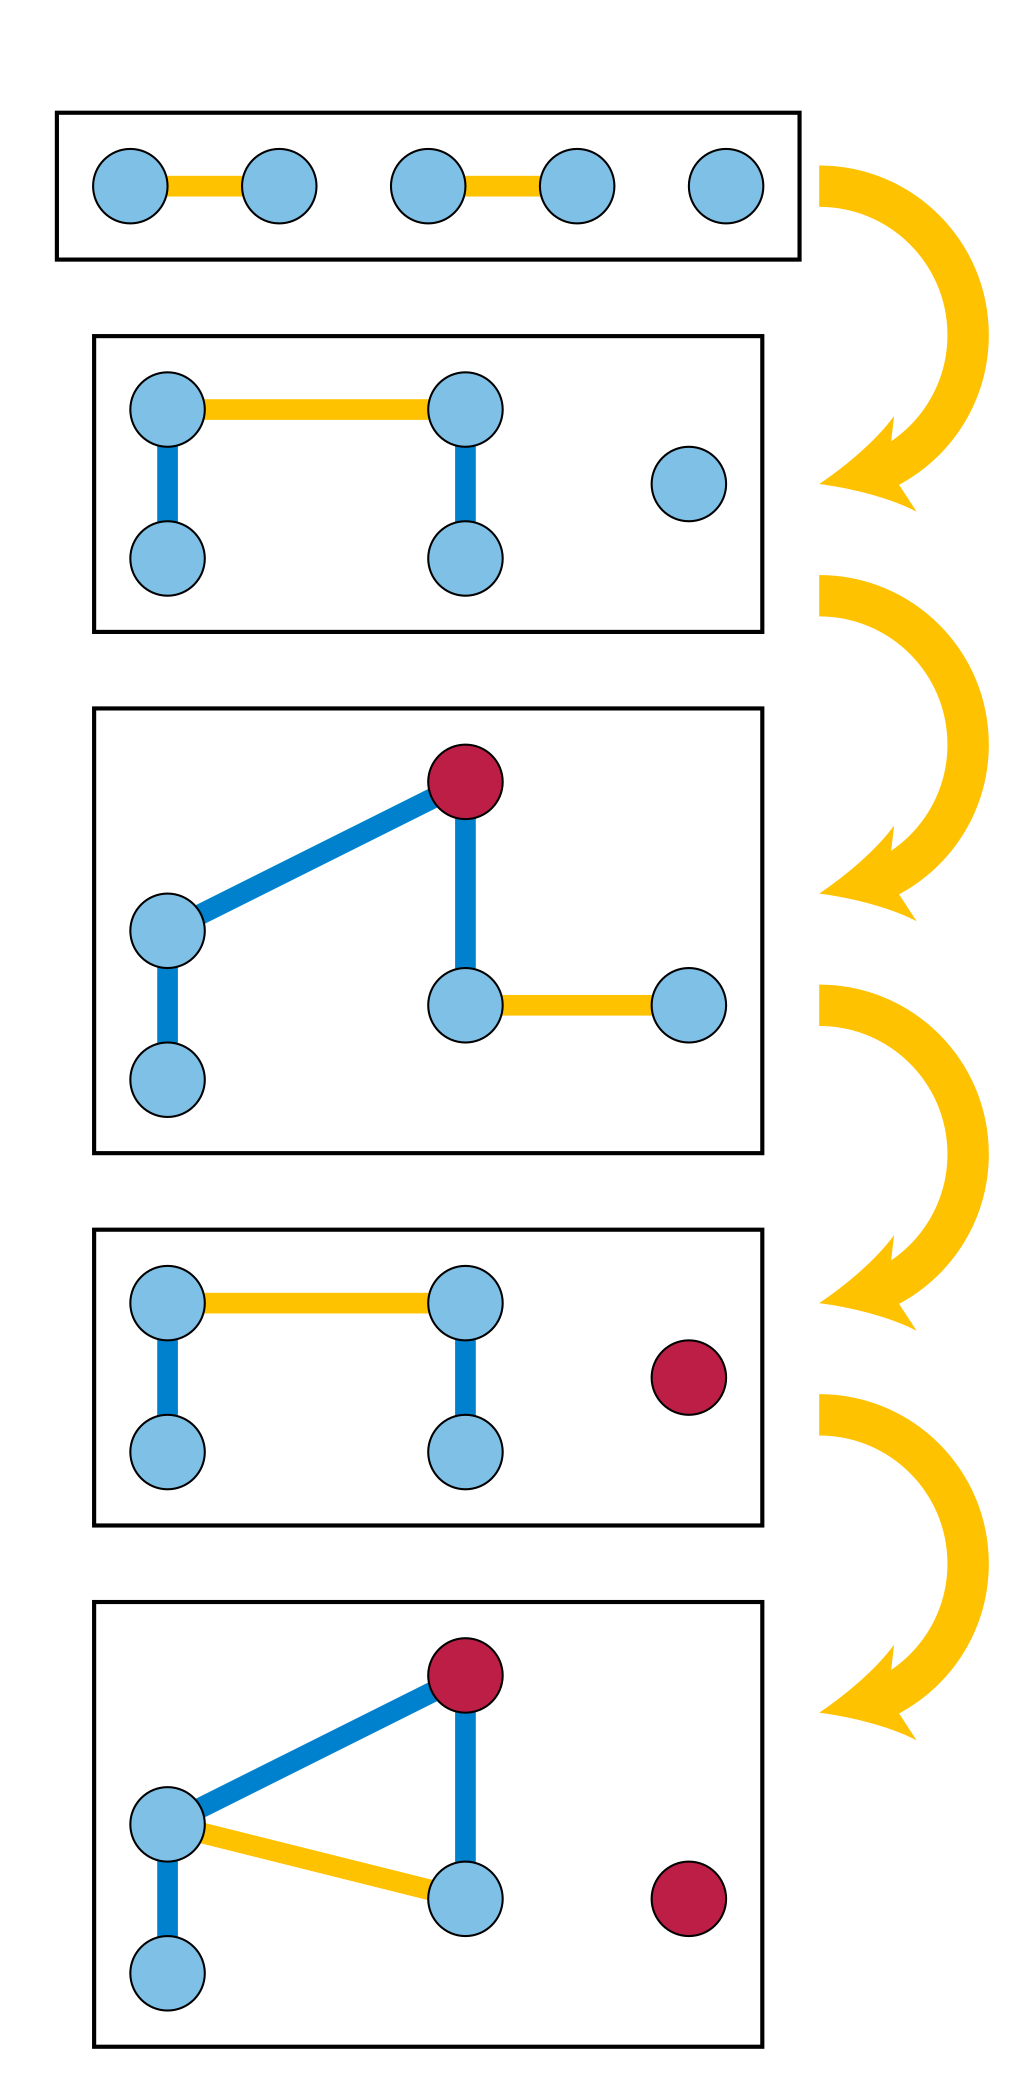
\includegraphics[width=0.5\columnwidth]{figures/Median_of_5.svg.png}
  \caption{Finding the median $i=3$ of $n=5$ values using six comparisons.}
  \label{fig:median_of_5}
\end{figure}
A good visual example is finding the median $i=3$ in a list of $n=5$ elements. Figure
(\ref{fig:median_of_5}) illustrate the search of the median using Hasse diagrams. Each step shows
the comparisons to be performed next as a yellow line. A Hasse diagram of the order of relation
found so far (smaller=lower, larger=higher) is shown as the blue lines. The red circles have already
found to be greater than three others and disqualified The red elements have already been determined
to be larger than three other elements and are therefore are disqualified as medians. The larger
element of the final comparison is the median. This is also the optimal algorithm for $i=3$ and
$n=5$.


\subsubsection{Solvability}
The solvability of a partial order can be determined in the following way. For each element, count
the elements that are smaller than it and count the elements that are larger than it. If there is an
element that is larger than $n-i$ elements and smaller than $i-1$ elements, this element is the
$i$-th largest element. Thus, the poset is solvable.


\section{Methods and Tools}
\subsection{Forward Search}
Forward Search starts with an empty Poset, i.e. one with entirely unknown ordering of its elements,
and recursively determines solvability of a given Poset within some bound by exhaustively searching
the results of all possible comparisons to be made unless it is already solved or we determine that
it cannot be solved within the alloted number of comparisons by some heuristic.

Between the two possible outcomes of a comparison we assume the worse, but since an algorithm is
free to choose which elements to compare we are looking for the most useful comparison, the one that
yields result Posets cheapest to solve themselves, still in terms of worst case outcome. The
algorithms output by the search program are built by saving the comparison that lead to this
cheapest to solve result.

To limit memory cost and allow further pruning we traverse the search tree depth first, reducing the
maximum number of comparisons alloted to child Posets to one less than the current best result
found. This premise is implemented by Minimax algorithms as shown in
figure~\ref{fig:minimax_search}.

We can drastically speed up this exploration by caching previous results, even with a simple usage
based ejection policy. Since the search always imposes an upper bound for the number of comparisons
to allow this also includes yet unsolved Posets, for which we note the currently known minimum.

It is optimal because of an inductive argument over the number of relative orders determined. An
already solved Poset obviously takes no further comparisons to solve. Then given an unsolved Poset
with all elements already too large or small excluded we must make at least one more comparison to
make progress. Since all Posets resulting from these comparisons must have more elements ordered
than the current one has we can assume as per induction that we know their optimal cost. Then we
cannot solve the Poset in less than the cost of the cheapest of these comparisons, plus one for the
comparison itself, hence the current Poset is also solved optimally.

It is also complete for a given upper bound, explainable through a similar inductive argument. If
the Poset is solvable within that bound then at least one of its possible comparisons must have both
outcomes be solvable within the bound lowered by one. Since the search only lowers the bound imposed
on its recursive descendants beyond that once at least one has been solved, we are also guaranteed
to find a solution for the original Poset if it exists within the bound.

\begin{figure}
  \begin{tikzpicture}[scale=0.8]
    \tiny
    \node (A1) at (0,0) {$\vdots$};
    \node (A2) at (2,0) {$\vdots$};
    \node (A3) at (3.5,0.4) {$\dots$};
    \node (A4) at (6,0) {$\vdots$};

    \node (B1) at (2,1) {MIN};

    \draw (B1) -- (A1) node[above,pos=0.6, xshift=-0.4cm] {$\{1,3\}$};
    \draw (B1) -- (A2) node[right, midway] {$\{1,4\}$};
    \draw (B1) -- (A4) node[right, pos=0.3, xshift=6mm] {$\{n \!- \! 1,n\}$};

    \node (C1) at (5,2) {MAX};
    \node (B2) at (7,1) {$\vdots$};

    \draw (C1) -- (B2) node[right, pos=0.3, xshift=4mm] {$(2,1)$};

    \draw (B1) -- (C1) node[left, pos=0.7, xshift=-4mm] {$(1,2)$};

    \node (D1) at (8,3) {MIN};
    \node (C2) at (8,2) {$\vdots$};
    \node (C3) at (8.7,2.3) {$\dots$};
    \node (C4) at (10,2) {$\vdots$};

    \draw (D1) -- (C1) node[left,pos=0.3,xshift=-3mm] {$\{1,2\}$};
    \draw (D1) -- (C2) node[left, midway, xshift=0.5mm] {$\{1,3 \! \}$};
    \draw (D1) -- (C4) node[right, pos=0.3,xshift=2mm] {$\{n \! - \! 1,n\}$};

  \end{tikzpicture}
  \caption{Minimax search algorithm} \label{fig:minimax_search}
\end{figure}

\subsection{Backward Search}

Backward search starts with a solved Poset, then repeatedly attempts to remove comparisons from its
frontier Posets such that the same Poset with the opposite comparison result is also found within
those already discovered.

Thus the number of iterations taken until a Poset is added to the frontier equals the number of
worst case comparisons needed to solve it, which means that the search terminates once the empty
Poset with the desired $n$ and $i$ is found.

The argument for the correctness is the number of comparisons we have found all Posets solvable
within them for, equal to the number of iterations of the search. If for a given Poset and a
comparison within it we have already discovered both results then their cost must be less than the
current number of iterations, so the Poset is solvable within that number and because this did not
hold true in a previous iteration the cost must also be optimal. And if a Poset is solvable within
that number of comparisons it must have at least one comparison with a result among the Posets
discovered in the previous iteration, as otherwise it would have to be solvable in less.

%%%%%%%%%%%%%%%%%%%%%%%%%%%%%%%%%%%%%%%%%%%%%%%%%%%%%%%%%%%%%%%%%
\subsubsection{Normalform}
Im Gegensatz zur Vorwärtssuche unterscheidet die Rückwärtssuche zwischen `kanonifizieren' und `normalisieren', wie folgt:
\begin{description}
  \item[kanonifizieren]
        überführt das Poset in eine \textbf{eindeutige} Normalform.
        Das `kanonifizieren` der Vorwärtssuche ist nicht eindeutig aus Performancegründen.
  \item[normalisieren]
        umfasst das reduzieren von Elementen, die nicht das $i$-kleinste Element sein können sowie das anschließende eindeutige `kanonifizieren'.
\end{description}

Um eine eindeutige Darstellung zu erhalten, wird zunächst geprüft, ob $2 * i < n$ gilt.
Sollte dies verletzt sein, werden alle Vergleiche umgedreht und $i := n - 1 - i$ gesetzt.
Ein mögliches Problem tritt auf, wenn $n - 1 = 2 * i$ gilt.
\begin{figure}
  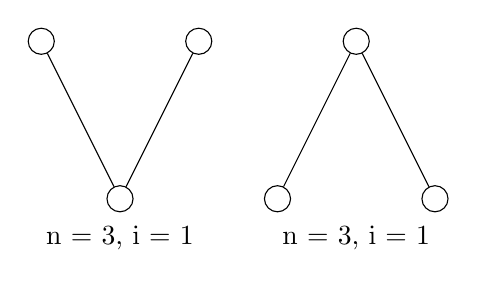
\begin{tikzpicture}
    \node[circle,draw=black] (A1) at (1, 0) {};
    \node[circle,draw=black] (A2) at (0, 2) {};
    \node[circle,draw=black] (A3) at (2, 2) {};

    \draw (A1) -- (A2) node {};
    \draw (A1) -- (A3) node {};
    \node (AL) at (1, -0.5) {n = 3, i = 1};


    \node[circle,draw=black] (B1) at (3 + 1, 2) {};
    \node[circle,draw=black] (B2) at (3 + 0, 0) {};
    \node[circle,draw=black] (B3) at (3 + 2, 0) {};

    \draw (B1) -- (B2) node {};
    \draw (B1) -- (B3) node {};
    \node (BL) at (3 + 1, -0.5) {n = 3, i = 1};
  \end{tikzpicture}
  \centering
  \caption{Problematischer Fall}
  \label{fig:backward_canonify_problematic}
\end{figure}
Wie in Abbildung~\ref{fig:backward_canonify_problematic} illustriert, sind beide Posets mittels nauty kanonifiziert und für beide Posets gilt  $2 * i < n$.
Offensichtlicherweise sind diese jedoch gleich, wenn alle Vergleiche umgekehrt werden.
Um dieses Problem zu beheben, wird jedes Poset, für das $n - 1 = i$ gilt normal kanonifiziert und anschließend werden alle Vergleiche umgedreht und es erneut kanonifiziert.
Anschließend wird deterministisch eins der beiden ausgewählt.

Da das Kanonifizieren für die Rückwärtssuche unumgänglich ist und während der Entwicklung ein Bottleneck darstellte, werden alle trivialen Fälle abgefangen und nur die restlichen mittels nauty kanonifiziert.
% TODO: Wie werden die trivialen Fälle abgefangen
In Abbildung~\ref{table:nauty-ratio} ist für $n = 12$ dargestellt, in wie vielen Prozent der Fälle das Programm nauty aufruft.

\begin{table}
  \begin{tabular}{l|l}
    $i$ & Nauty-Ratio \\
    \hline
    $0$ & $0\%$       \\
    $1$ & $10.12\%$   \\
    $2$ & $7.96\%$    \\
    $3$ & $3.67\%$    \\
    $4$ & $2.03\%$    \\
    $5$ & $1.49\%$
  \end{tabular}
  \centering
  \caption{Prozentwert der Aufrufe an `nauty' zum kanonifizieren}
  \label{table:nauty-ratio}
\end{table}

\subsubsection{Algorithmus}
Eingabe für den Rückwärtssuche stellen die Parameter $n$ und $i$ dar.
Die Rückwärtssuche startet bei dem kleinsten gelösten Poset und berechnet iterativ alle Posets, die in $1, 2, 3, \dots$ Vergleichen gelöst werden können, bis das leere Poset der Größe $n$ und $i$ gefunden wird.
Das kleinste gelöste Poset ist das Poset, das aus einem Element besteht und keinen Vergleichen besteht.
Das leere Poset ist das Poset, das $n$ Elemente hat, das $i$-kleinste Element gesucht wird und keine Vergleiche umfasst.
Verallgemeinert sei $A_k$ die Menge aller Posets, die in $k$ Vergleichen lösbar ist (in diesem Fall besteht $A_0$ nur aus dem kleinsten gelösten Poset).
Im Folgenden berechnet die Rückwärtssuche für jedes Posets in der Menge $A_k$, die entsprechenden Nachfolger.
Ein Nachfolger von Poset $p$ hat folgende Eigenschaften:
\begin{itemize}
  \item es ist vollständig normalisiert
  \item es ist nicht in einer vorherigen Runde gefunden (da es sonst in weniger Vergleichen lösbar wäre)
  \item es existiert ein Vergleich $(i, j)$, durch deren Hinzunahme und anschließender Normalisierung wieder Poset $p$ resultiert und durch Hinzunahme des Umkehrvergleichs $(j, i)$ und anschließender Normalisierung wieder ein bereits gefundenes Poset resultiert
\end{itemize}
Die Menge aller Nachfolger bildet die Menge $A_{k + 1}$.

\subsubsection{Nachfolgerberechnung}
% um ein Poset `q' zu ``enlarge_and_remove_less'':
% 1. ``enlarge''-Schritt
% 2. ``remove-less''-Schritt
% 3. ``enlarge2''-Schritt

1. Die Rückwärtssuche basiert auf dem Entfernen von Vergleichen. Da es Posets gibt (und um alle Posets zu erwischen), wird zunächst das Poset `q' mit Größe `n' und dem `k'-kleinsten Element vergrößert. Das heißt es wird ein Dummy-Element eingefügt. Um dies zu konkretisieren, berechnet dieser Schritt alle Posets, die Größe `n + 1' haben und entweder das `k' oder `k + 1'-kleinste Element gesucht wird (dies liegt daran, dass das Dummy-Element unter oder über unserem gesuchten k-kleinsten Element eingefügt wird, wodurch sich das ursprüngliche k-kleinste Element eventuell verschiebt). Des Weiteren müssen entsprechende Vergleiche eingefügt werden, sodass das Dummy-Element nicht das `k' bzw. `k + 1'-kleinste Element sein kann.
Letztlich sollte sichergestellt werden, dass alle Posets in einer eindeutigen kanonifizierten Normalform für den nächsten Schritt umgewandelt werden.
Die aktuelle Menge der gespeicherten Posets umfasst alle neu berechneten sowie das ursprüngliche Poset `q'.

2. In diesem Schritt wird ein beliebiger Vergleich `(i, j)' entfernt. Eine Schwierigkeit stellen hierbei die transitiven Vergleiche dar: \\
Zum Beispiel können Poset (2) und (3) durch das Entfernen des Vergleichs vom mittleren zum unteren Element entstehen, wie in Abbildung~\ref{fig:backward_problematic} veranschaulicht. \\
\begin{center}
  \begin{figure}
    \begin{tikzpicture}
      \node[circle,draw=black] (A1) at (0, 0) {};
      \node[circle,draw=black] (A2) at (0, 1) {};
      \node[circle,draw=black] (A3) at (0, 2) {};

      \draw (A1) -- (A2) node {};
      \draw (A2) -- (A3) node {};
      \node (A) at (0, -1) {(1)};


      \node[circle,draw=black] (B1) at (3 + 0, 0) {};
      \node[circle,draw=black] (B2) at (3 + 0, 2) {};
      \node[circle,draw=black] (B3) at (3 + 1, 1) {};

      \draw (B1) -- (B2) node {};
      \node (B) at (3 + 0.5, -1) {(2)};


      \node[circle,draw=black] (C1) at (6 + 1, 2) {};
      \node[circle,draw=black] (C2) at (6 + 0, 0) {};
      \node[circle,draw=black] (C3) at (6 + 2, 0) {};

      \draw (C1) -- (C2) node {};
      \draw (C1) -- (C3) node {};
      \node (C) at (6 + 1, -1) {(3)};
    \end{tikzpicture}
    \caption{Problematischer Fall} \label{fig:backward_problematic}
  \end{figure}
\end{center}
Um dieses Problem zu lösen, werden alle möglichen Nachfolger berechnet.

Eine weiter Optimierung ist hierbei nur Vergleiche zu entfernen, die im 1. Schritt eingefügt wurden oder normal.

3. Anschließend werden alle Posets gesucht, die folgenden Bedingung erfüllen:



- Menge B := alle Posets in A kanonifiziert (ACHTUNG: man muss sich merken, welches Element neu hinzugekommen ist)
- Menge C := alle Posetes, die sich ergeben, wenn aus `q` ODER einem Poset aus B ein beliebiger Vergleich entfernt wird
- hierbei kann das entfernen eines beliebigen Vergleiches mehrere Posets produzieren, da nicht klar ist, wann welcher transitive Vergleich eingefügt wurde
- Vergleich darf nur entfernt werden, wenn dadurch nicht ein Element wegreduziert werden könnte
- kanonifiziere diese Menge anschließend
- berechne iteraitv (vergrößere entweder nur n ODER n und k) anschließend noch alle größeren Posets, die
- das hinzugefügte Element durch transitive Verlgeiche wegoptimiert werden könnte
- durch hinzufügen

\subsubsection{Parallelisierung}
Die Rückwärtssuche kann sehr gut parallelisiert werden, indem die Berechnung der Nachfolger parallel passiert. Wie in Abbildung~\ref{table:backward-parallel} beispielhaft für $n = 10, i = 4$ dargestellt, skaliert die Rückwärtssuche relativ gut mit der Anzahl der Kerne.

\begin{table}
  \begin{tabular}{l|l|l}
    Anzahl Kerne & Zeit in s & Parallelitätsfaktor \\
    \hline
    $1$          & $43.070$  & $?$                 \\ % TODO: diese Werte sind bis jetzt nur dummy-werte
    $2$          & $25.038$  & $?$                 \\
    $3$          & $18.925$  & $?$                 \\
    $4$          & $16.307$  & $?$                 \\
  \end{tabular}
  \centering
  \caption{Faktor der Parallelisierung für $n = 10, i = 4$}
  \label{table:backward-parallel}
\end{table}

%%%%%%%%%%%%%%%%%%%%%%%%%%%%%%%%%%%%%%%%%%%%%%%%%%%%%%%%%%%%%%%%%

\subsection{Bidirectional Search}

\subsection{$\alpha$-$\beta$-pruning}

\subsection{Compatible Posets}

\section{Results}

\begin{table}
  \centering
  \begin{tabular}{c|cccccccc}
    $n$ & \multicolumn{8}{c}{$i$}                                   \\
        & 0                       & 1  & 2  & 3  & 4  & 5  & 6  & 7 \\ \hline
    1   & 0                                                         \\
    2   & 1                                                         \\
    3   & 2                       & 3                               \\
    4   & 3                       & 4                               \\
    5   & 4                       & 6  & 6                          \\
    6   & 5                       & 7  & 8                          \\
    7   & 6                       & 8  & 10 & 10                    \\
    8   & 7                       & 9  & 11 & 12                    \\
    9   & 8                       & 11 & 12 & 14 & 14               \\
    10  & 9                       & 12 & 14 & 15 & 16               \\
    11  & 10                      & 13 & 15 & 17 & 18 & 18          \\
    12  & 11                      & 14 & 17 & 18 & 19 & 20          \\
    13  & 12                      & 15 & 18 & 20 & 21 & 22 & 23     \\
    14  & 13                      & 16 & 19 & 21 & 23 & 24 & 25     \\
    15  & 14                      & 17 & 20 & 23 & 24 & 26 & 26 & ? \\
  \end{tabular}
  \caption{The minimum amount of comparisons needed to select the $i+1$-th smallest of $n$}
  \label{table:num_comparisons}
\end{table}

See Table~\ref*{table:num_comparisons}.


\subsection{Search evaluation}
\subsubsection{Backward search}
\subsubsection{bidirectional search}
\subsubsection{forward search}

\subsection{Algorithmic improvements}

\subsubsection{Heuristics}

We used multiple heuristics to estimate if a poset is solvable in a given number of comparisons.
These heuristics are used to reject posets, that are not solvable in the given number of comparisons.
This reduces the number of posets that need to be searched.

The first heuristic uses the number of compatible posets.
We use the fact, that the number of comparisons needed to solve a poset is less than the base two logarithm of the number of compatible posets,
to estimate if a poset is solvable.

The second heuristic searches for two elements which have not beend compared yet.
One of these two elements is maximal and has at least two elements smaller than it,
and the other element is minimal and has at least two elements greater than it.
We then construct a new poset with a comparison added, where the minimal element is smaller than the maximal.
The new poset is then searched for a solution using the forward seach described above.
If the new poset is found to be solvable in the given number of comparisons, we estimate that the original poset is also solvable.
If the new poset is not solvable, we estimate the original is not solvable either.
This heuristic can be slightly improved by maximising the number of elements smaller than the maximal element and greater than the minimal element.

\subsubsection{Triangular Adjacency Matrix}
Storing an adjacency matrix for a poset of size $n$ takes $n^2 - n$ bits, one for each possible relation.
The diagonal does not need to be stored, as an element can not be smaller than itself.

By canonifying the poset, the elements can be sorted in a way such that each element is not smaller than any element before it.
This property can be used to reduce the adjacency matrix to a triangular matrix, which can then be stored using $\frac{n^2 - n}{2}$ bits.
It can also simplify some algorithms, for example calculating the number of compatible posets.

\subsubsection{Multithreading}

\section{Conclusion}
We found a better solution hooray!
These are points we'd like to take into account for further research


\appendices
\section{Proof of the First Zonklar Equation}
Appendix one text goes here.
\section{}
Appendix two text goes here.


\ifCLASSOPTIONcompsoc
  \section*{Acknowledgments}
\else
  \section*{Acknowledgment}
\fi


The authors would like to thank...

\ifCLASSOPTIONcaptionsoff
  \newpage
\fi


\bibliographystyle{IEEEtran}
\bibliography{biblio.bib}
\end{document}